\chapter{Trabajo, energía y energía potencial}\label{ch:b1:work-and-energy}

Un ciclista deja de pedalear en lo alto de una cuesta y llega abajo con
una rapidez que depende del desnivel, no de la forma de la carretera.
Quien salta con una cuerda elástica cae sesenta metros y se detiene, un
instante, exactamente donde el tirón de la cuerda se ha comido toda la
rapidez que le había dado la caída. Un átomo de hidrógeno ligado a uno de
cloro vibra en un pozo cuya profundidad es la energía que cuesta romper la
molécula. En cada caso se intercambia un solo número entre formas ---
movimiento, altura, alargamiento, enlace --- y, sumado, no cambia. Este
capítulo construye esa contabilidad a partir de la segunda ley de Newton:
\omterm{def:b1:work-and-energy:work}{trabajo} y potencia, el \omterm{thm:b1:work-and-energy:ke}{teorema de la energía cinética}, las \omterm{def:b1:work-and-energy:conservative}{energías
potenciales} de las fuerzas que las admiten y la \omterm{thm:b1:work-and-energy:em}{conservación de la energía
mecánica}, que convierte muchos problemas de dinámica en un renglón de
álgebra y explica, por la forma de un \omterm{def:b1:work-and-energy:turning}{pozo de potencial}, qué posiciones
son estables.

\begin{omfigure}
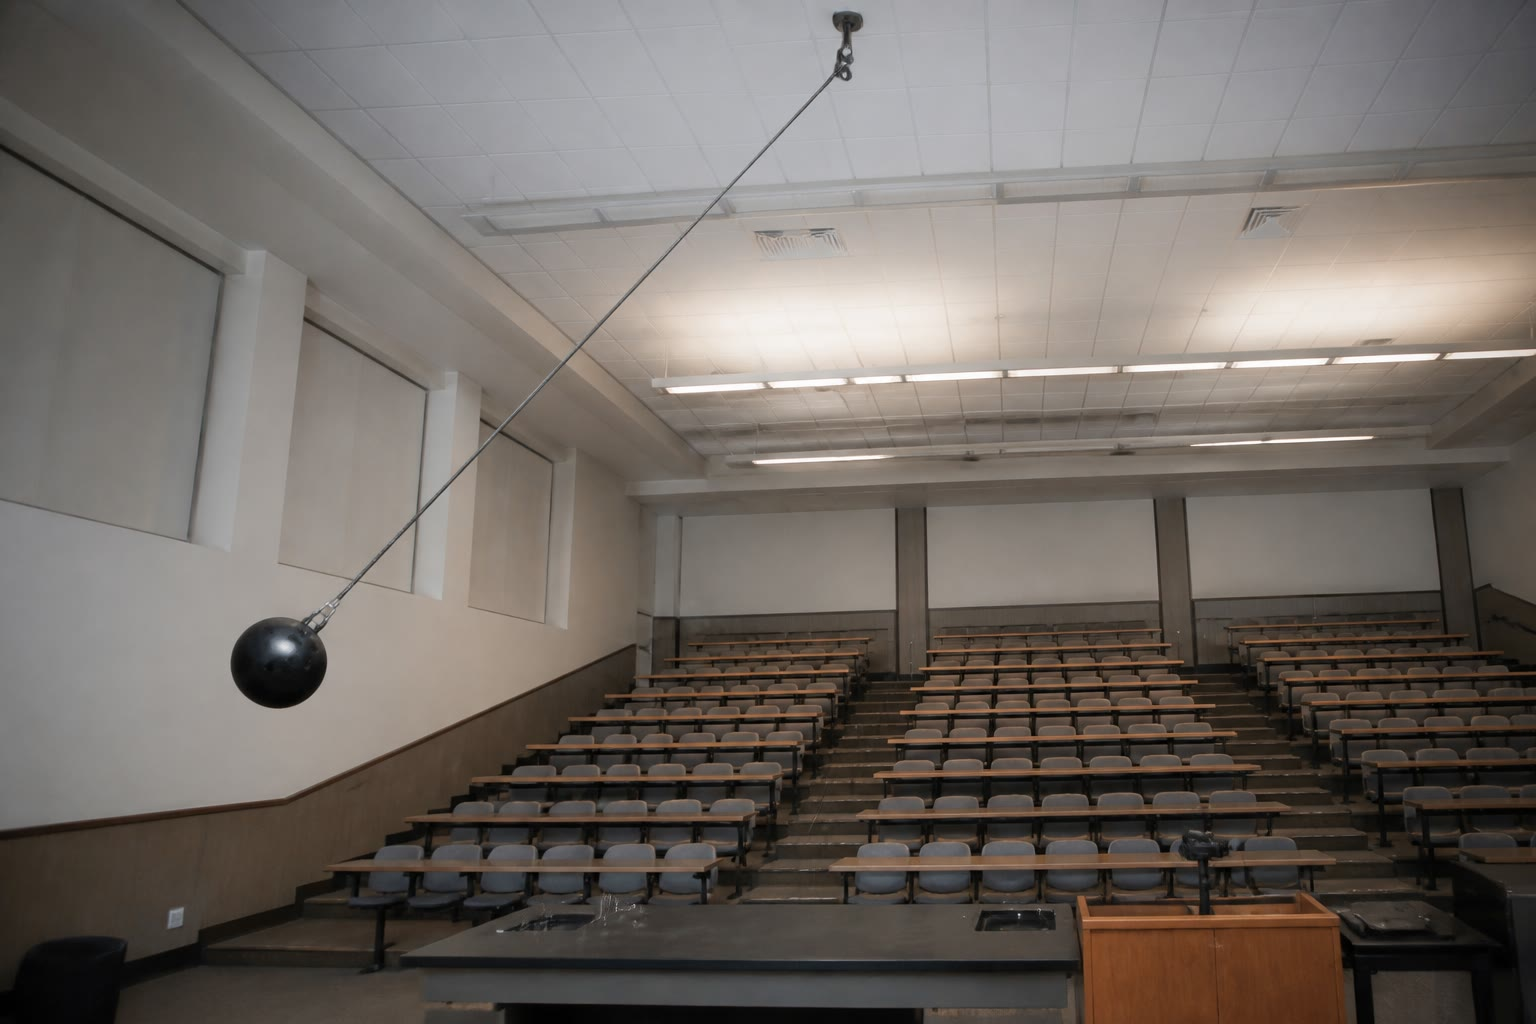
\includegraphics[width=0.58\linewidth]{images/book3/ai/b3-13-lecture-hall-pendulum.jpg}

{\small El péndulo del profesor: soltada desde la nariz, la bola de bolos vuelve a la nariz y no más allá --- la \omterm{thm:b1:work-and-energy:em}{energía mecánica} se conserva, y nunca se supera.}
\end{omfigure}

\section{Potencia y trabajo}

\begin{definition}[Potencia y trabajo de una fuerza]\label{def:b1:work-and-energy:work}
\index{potencia (de una fuerza)}\index{trabajo}
La \emph{potencia} de una fuerza $\vect F$ que actúa sobre un punto que se
mueve con velocidad $\vect v$ es
\[
\mathcal P = \vect F\cdot\vect v \qquad (\text{vatios}),
\]
y su \emph{trabajo} entre los instantes $t_1$ y $t_2$ (posiciones $A$ y
$B$) es la potencia acumulada,
\[
W_{A\to B} = \int_{t_1}^{t_2}\vect F\cdot\vect v\,\dd t
= \int_A^B \vect F\cdot\dd\vect\ell \qquad (\text{julios}),
\]
la suma de los \emph{trabajos elementales} $\delta W = \vect F\cdot\dd\vect\ell$
a lo largo de los desplazamientos elementales $\dd\vect\ell = \vect v\,\dd t$
de la \omterm{def:b1:point-kinematics:frame}{trayectoria}. El trabajo es positivo si la fuerza empuja en el
sentido del movimiento (\emph{motor}), negativo si se opone
(\emph{resistente}), y nulo si es perpendicular.
\end{definition}

\begin{proposition}[Trabajos que se encuentran]\label{prop:b1:work-and-energy:works}
\begin{itemize}
  \item Fuerza constante: $W_{A\to B} = \vect F\cdot\vect{AB}$, sea cual
        sea el camino. Peso: $W = mg(z_A - z_B)$, con $z$ contada hacia arriba.
  \item Resorte de rigidez $k$, del alargamiento $x_A$ al $x_B$:
        $W = \tfrac12 k(x_A^2 - x_B^2)$.
  \item \omterm{prop:b1:newton-dynamics:friction}{Reacción normal} de una superficie fija, tensión de un hilo sobre
        un cuerpo que se mueve perpendicularmente a él: $W = 0$ (fuerza
        $\perp$ desplazamiento).
  \item Rozamiento cinético y arrastre: $W < 0$ siempre (la fuerza se
        opone al movimiento relativo) y depende de la longitud del camino.
\end{itemize}
\end{proposition}

\begin{proof}
$\vect F$ constante: $\int\vect F\cdot\dd\vect\ell = \vect F\cdot\int\dd\vect\ell
= \vect F\cdot\vect{AB}$; con $\vect F = -mg\vect e_z$, $\vect F\cdot\vect{AB}
= -mg(z_B - z_A)$. Resorte: $\vect F\cdot\dd\vect\ell = -kx\,\dd x$, y
$\int_{x_A}^{x_B}-kx\,\dd x = \tfrac12 k(x_A^2 - x_B^2)$. Rozamiento: $\vect T
= -\mu N\vect v/v$, luego $\vect T\cdot\vect v = -\mu Nv < 0$.
\end{proof}

\begin{omfigure}
\begin{tikzpicture}[font=\small, x=1cm, y=1cm]
  \draw[omDef, thick, domain=0:6, samples=60] plot (\x, {0.35*\x + 0.9*sin(deg(0.7*\x))});
  \fill (0,0) circle (1.4pt) node[below] {$A$};
  \fill (6,{2.1+0.9*sin(deg(4.2))}) circle (1.4pt) node[right] {$B$};
  % point at x=2.4: y = 0.84+0.9*sin(96.3deg)=0.84+0.894=1.734 ; slope 0.35+0.63cos(96.3)=0.35-0.069=0.28
  \coordinate (M) at (2.4,1.734);
  \fill[omThm] (M) circle (1.6pt); \node[above left] at (M) {$M$};
  \draw[-Stealth, omThm, very thick] (M) -- ++(1.1,0.31) node[right] {$\dd\vect\ell$};
  \draw[-Stealth, omProp, very thick] (M) -- ++(1.4,-0.9) node[below right] {$\vect F$};
  \draw ($(M)+(0.55,0.15)$) arc (15.6:-32.7:0.57); \node at ($(M)+(0.85,-0.12)$) {$\alpha$};
  \node[omExo, font=\footnotesize] at (3.6,3.4) {$\delta W = \vect F\cdot\dd\vect\ell = F\,\dd\ell\cos\alpha$};
\end{tikzpicture}

{\small El \omterm{def:b1:work-and-energy:work}{trabajo} elemental de una fuerza a lo largo de un pequeño
desplazamiento de su punto de aplicación: solo trabaja la componente de
$\vect F$ en la dirección del movimiento. Sumado a lo largo del camino de
$A$ a $B$, da $W_{A\to B}$.}
\end{omfigure}

\section{El teorema de la energía cinética}

\begin{theorem}[Teoremas de la energía cinética y de la potencia]\label{thm:b1:work-and-energy:ke}
\index{energía cinética}\index{teorema de la energía cinética}
En un \omterm{thm:b1:newton-dynamics:laws}{sistema inercial}, la \emph{\omterm{thm:b1:work-and-energy:ke}{energía cinética}} $E_k = \tfrac12 mv^2$
de un \omterm{def:b1:point-kinematics:frame}{punto material} cumple
\[
\frac{\dd E_k}{\dd t} = \sum\mathcal P_i = \Big(\sum\vect F_i\Big)\cdot\vect v,
\qquad
E_k(B) - E_k(A) = \sum_i W_{i,A\to B}:
\]
la variación de \omterm{thm:b1:work-and-energy:ke}{energía cinética} entre dos posiciones es igual al \omterm{def:b1:work-and-energy:work}{trabajo}
total de todas las fuerzas aplicadas a lo largo del camino.
\end{theorem}

\begin{proof}
Multiplíquese escalarmente la segunda ley de Newton por $\vect v$: $m\vect a\cdot\vect v =
\tfrac{\dd}{\dd t}(\tfrac12 m\vect v\cdot\vect v) = \dd E_k/\dd t$, mientras que
$(\sum\vect F_i)\cdot\vect v = \sum\mathcal P_i$. Intégrese en el tiempo.
\end{proof}

\begin{example}[Distancia de frenado]\label{ex:b1:work-and-energy:braking}
Un coche de \qty{1000}{kg} a \qty{100}{km/h} ($E_k = \qty{386}{kJ}$)
frenado por una fuerza constante de \qty{7.0}{kN} se detiene tras
$d = E_k/F = \qty{55}{m}$: la distancia crece con el \emph{cuadrado} de la
rapidez. Como la fuerza máxima de frenado vale $\mu_smg$
(\cref{ch:b1:newton-dynamics}), la distancia de parada mínima es
$v^2/2\mu_sg$ sea cual sea la masa del coche --- y se duplica en calzada
mojada, donde $\mu_s$ se reduce a la mitad.
\end{example}

\section{Fuerzas conservativas y energía potencial}

\begin{definition}[Fuerza conservativa; energía potencial]\label{def:b1:work-and-energy:conservative}
\index{fuerza conservativa}\index{energía potencial}
Una fuerza es \emph{conservativa} si su \omterm{def:b1:work-and-energy:work}{trabajo} entre dos puntos no
depende del camino seguido. De forma equivalente, existe una función de
la posición, la \emph{energía potencial} $E_p$, tal que
\[
W_{A\to B} = E_p(A) - E_p(B) = -\Delta E_p ,
\qquad \delta W = -\dd E_p ,
\]
con $E_p$ definida salvo una constante aditiva (una elección de origen).
\end{definition}

\begin{proposition}[La fuerza a partir de la energía potencial]\label{prop:b1:work-and-energy:gradient}
\index{gradiente}
Una \omterm{def:b1:work-and-energy:conservative}{fuerza conservativa} deriva de su \omterm{def:b1:work-and-energy:conservative}{energía potencial}:
\[
\vect F = -\overrightarrow{\operatorname{grad}}\,E_p
= -\frac{\partial E_p}{\partial x}\,\vect e_x
- \frac{\partial E_p}{\partial y}\,\vect e_y
- \frac{\partial E_p}{\partial z}\,\vect e_z ,
\]
y en una dimensión $F_x = -\dd E_p/\dd x$: la fuerza apunta hacia las
\omterm{def:b1:work-and-energy:conservative}{energías potenciales} decrecientes, ``cuesta abajo'' en la gráfica de $E_p$.
\end{proposition}

\begin{proof}
$\delta W = F_x\dd x + F_y\dd y + F_z\dd z = -\dd E_p = -(\partial_xE_p\,\dd x
+ \partial_yE_p\,\dd y + \partial_zE_p\,\dd z)$ para todo desplazamiento:
identifíquense los coeficientes (la diferencial de una función de varias
variables, del curso de matemáticas).
\end{proof}

\begin{proposition}[Las energías potenciales habituales]\label{prop:b1:work-and-energy:eps}
\index{energía potencial!gravitatoria}\index{energía potencial!elástica}
\begin{itemize}
  \item Peso: $E_p = mgz + \text{cte}$ (con $z$ hacia arriba).
  \item Resorte: $E_p = \tfrac12 k(\ell - \ell_0)^2 + \text{cte}$.
  \item Gravitación newtoniana de una masa $M$: $E_p = -GMm/r + \text{cte}$,
        con la constante elegida normalmente para que $E_p \to 0$ en el
        infinito.
  \item Fuerza electrostática sobre una carga $q$ en un potencial $V$:
        $E_p = qV$ (\cref{ch:b1:potential-capacitors}).
\end{itemize}
El rozamiento cinético y el arrastre fluido \emph{no} son conservativos
(su \omterm{def:b1:work-and-energy:work}{trabajo} depende del camino y es siempre negativo).
\end{proposition}

\begin{proof}
Cada una se lee en los \omterm{def:b1:work-and-energy:work}{trabajos} de \cref{prop:b1:work-and-energy:works}:
$W = -\Delta E_p$. Para la gravitación, $\vect F = -GMm/r^2\,\vect e_r$ y
$\delta W = -GMm\,\dd r/r^2 = -\dd(-GMm/r)$.
\end{proof}

\section{Energía mecánica}

\begin{theorem}[Energía mecánica]\label{thm:b1:work-and-energy:em}
\index{energía mecánica}\index{conservación de la energía mecánica}
Sea $E_m = E_k + E_p$ la \emph{\omterm{thm:b1:work-and-energy:em}{energía mecánica}}, donde $E_p$ es la suma
de las \omterm{def:b1:work-and-energy:conservative}{energías potenciales} de las \omterm{def:b1:work-and-energy:conservative}{fuerzas conservativas}. Entonces
\[
\Delta E_m = W_{\text{nc}} ,
\]
el \omterm{def:b1:work-and-energy:work}{trabajo} total de las fuerzas no conservativas. Si estas no trabajan
(sin rozamiento, o con fuerzas de ligadura perpendiculares al
movimiento), $E_m$ se \emph{conserva}: el movimiento es \emph{conservativo}.
\end{theorem}

\begin{proof}
$\Delta E_k = W_{\text{c}} + W_{\text{nc}} = -\Delta E_p + W_{\text{nc}}$.
\end{proof}

\begin{method}[Usar la energía]\label{met:b1:work-and-energy:method}
Cuando un problema pide una \emph{rapidez en una posición} (no un tiempo,
no una fuerza), pruébese primero con la energía:
\begin{enumerate}
  \item enumérense las fuerzas; véase cuáles trabajan y cuáles son
        conservativas;
  \item escríbase $E_m$ en las dos posiciones, con un origen claro para $E_p$;
  \item iguálense (añadiendo $W_{\text{nc}}$ si actúa el rozamiento) y
        despéjese la rapidez o la posición buscadas.
\end{enumerate}
La energía nunca da el tiempo ni las fuerzas de ligadura; para eso hay que
volver a la ley de Newton --- a menudo con la rapidez que la energía acaba de dar.
\end{method}

\begin{example}[La ley de rapidez del rizo]\label{ex:b1:work-and-energy:loop}
En el rizo sin rozamiento de \cref{pb:b1:point-kinematics:1}, la reacción
de la vía es normal al movimiento y no trabaja: $E_m$ se conserva. Con
$z = R(1 - \cos\theta)$ sobre el punto más bajo, $\tfrac12 mv^2 + mgR(1 -
\cos\theta) = \tfrac12 mv_0^2$: la ley de rapidez $v^2 = v_0^2 - 2gR(1 -
\cos\theta)$ que allí se usó, ahora deducida en un renglón. La rapidez
mínima de entrada $\sqrt{5gR}$ se sigue entonces de la condición en lo
alto $v^2 \geq gR$ de \cref{ex:b1:newton-dynamics:circles}.
\end{example}

\begin{example}[Energía perdida en el rozamiento]\label{ex:b1:work-and-energy:friction}
Un bloque desliza por una pendiente de ángulo $\alpha$ y altura $h$ con
rozamiento cinético $\mu_d$: $W_{\text{nc}} = -\mu_dmg\cos\alpha \times
h/\sin\alpha = -\mu_dmgh\cot\alpha$, luego $\tfrac12 mv^2 = mgh(1 - \mu_d\cot\alpha)$.
Para $h = \qty{2.0}{m}$, $\alpha = 30^\circ$ y $\mu_d = 0.20$: $v =
\qty{5.1}{m/s}$ en lugar de $\qty{6.3}{m/s}$; un tercio de la \omterm{def:b1:work-and-energy:conservative}{energía
potencial} se convirtió en calor.
\end{example}

\section{Equilibrio, estabilidad y retratos de fases}

\begin{proposition}[Equilibrio y estabilidad en una dimensión]\label{prop:b1:work-and-energy:stability}
\index{equilibrio!estable, inestable}\index{pequeñas oscilaciones}
Un \omterm{def:b1:point-kinematics:frame}{punto material} que se mueve sobre un eje bajo una \omterm{def:b1:work-and-energy:conservative}{fuerza conservativa}
de \omterm{def:b1:work-and-energy:conservative}{energía potencial} $E_p(x)$:
\begin{itemize}
  \item está en \emph{equilibrio} en $x_0$ si y solo si $F(x_0) = -E_p'(x_0) = 0$:
        en los extremos de $E_p$;
  \item el equilibrio es \emph{estable} si $E_p$ tiene allí un mínimo
        local ($E_p''(x_0) > 0$): un desplazamiento pequeño produce una
        fuerza recuperadora; es \emph{inestable} en un máximo;
  \item cerca de un equilibrio estable, los movimientos pequeños son
        armónicos, con
        \[
        \omega_0^2 = \frac{E_p''(x_0)}{m} .
        \]
\end{itemize}
\end{proposition}

\begin{proof}
Fórmula de Taylor (curso de matemáticas): $E_p(x) \approx E_p(x_0) +
\tfrac12 E_p''(x_0)(x - x_0)^2$, luego $F \approx -E_p''(x_0)(x - x_0)$ y
$m\ddot x = -E_p''(x_0)(x - x_0)$ --- un resorte de rigidez $E_p''(x_0)$.
Para $E_p'' < 0$ la ``rigidez'' es negativa: alejamiento exponencial.
\end{proof}

\begin{omfigure}
\begin{tikzpicture}
\begin{axis}[omaxis, axis x line=bottom, axis y line=left, width=10.5cm, height=5.8cm, xlabel={$x$}, ylabel={$E_p$},
    xlabel style={at={(axis description cs:0.5,-0.06)}, anchor=north},
    xmin=-2.3, xmax=2.5, ymin=-1.5, ymax=1.6, xtick={-1,1}, xticklabels={$-a$,$a$}, ytick=\empty]
  \addplot[omDef, thick, domain=-2.15:2.15, samples=200] {x^4 - 2*x^2 + 0.3*x};
  \addplot[omThm, dashed, domain=-2.3:2.5, samples=2] {-0.45};
  \addplot[omExo, dashed, domain=-2.3:2.5, samples=2] {0.9};
  \node[omThm, font=\footnotesize, anchor=east] at (axis cs:2.45,-0.3) {$E_1$};
  \node[omExo, font=\footnotesize, anchor=east] at (axis cs:2.45,1.05) {$E_2$};
  \node[font=\footnotesize, below] at (axis cs:-1.08,-0.7) {estable};
  \node[font=\footnotesize, above] at (axis cs:0.08,0.08) {inestable};
  \node[font=\footnotesize, below] at (axis cs:0.97,-1.1) {estable};
  \draw[Stealth-Stealth, omThm] (axis cs:-1.56,-0.45) -- (axis cs:-0.47,-0.45);
  \draw[Stealth-Stealth, omThm] (axis cs:0.42,-0.45) -- (axis cs:1.48,-0.45);
\end{axis}
\end{tikzpicture}

{\small Un paisaje de potencial unidimensional: los mínimos son
equilibrios estables y el máximo uno inestable. Un punto de energía $E_1$
por debajo de la barrera queda atrapado en un pozo entre dos \emph{\omterm{def:b1:work-and-energy:turning}{puntos
de retroceso}} (donde $E_p = E_1$, flechas) y oscila; con $E_2$ por encima
de la barrera pasa libremente de un pozo al otro.}
\end{omfigure}

\begin{definition}[Puntos de retroceso; movimiento ligado y libre]\label{def:b1:work-and-energy:turning}
\index{punto de retroceso}\index{movimiento ligado}\index{pozo de potencial}\index{barrera de potencial}
Para un movimiento unidimensional conservativo de energía $E_m$, el punto
solo puede estar donde $E_p(x) \leq E_m$ (ya que $E_k \geq 0$); los puntos
en los que $E_p = E_m$ son \emph{puntos de retroceso}, donde la velocidad
se anula y se invierte. Atrapado entre dos puntos de retroceso en un
\emph{pozo de potencial}, el movimiento es \emph{ligado} y periódico; si
puede alcanzar el infinito, es \emph{libre}; una \emph{barrera de
potencial} más alta que $E_m$ no puede atravesarse.
\end{definition}

\begin{definition}[Retrato de fases]\label{def:b1:work-and-energy:phase}
\index{retrato de fases}
El \emph{retrato de fases} de un movimiento unidimensional es la familia
de curvas que traza el punto $(x, \dot x)$ en el \emph{plano de fases}.
Para un sistema conservativo, cada curva es una línea de nivel
$\tfrac12 m\dot x^2 +
E_p(x) = E_m$: curvas cerradas alrededor de los equilibrios estables
(oscilaciones), curvas abiertas para el movimiento libre y, pasando por
los equilibrios inestables, las \emph{separatrices} que dividen ambos
tipos. Las curvas se recorren en sentido horario ($\dot x > 0$ significa
$x$ creciente) y nunca se cortan.
\end{definition}

\begin{omfigure}
\begin{tikzpicture}
\begin{axis}[omaxis, width=11cm, height=6.2cm, xlabel={$\theta$}, ylabel={$\dot\theta/\omega_0$},
    xmin=-7.2, xmax=7.2, ymin=-2.6, ymax=2.6, xtick={-6.283,-3.1416,0,3.1416,6.283},
    xticklabels={$-2\pi$,$-\pi$,$0$,$\pi$,$2\pi$}, ytick={-2,2}]
  % closed curves: thetadot^2 = 2(e - (1 - cos theta)) with e<2 ; thetadot = ±sqrt(2(e-1+cos))
  \foreach \e/\tm in {0.3/0.795, 1.0/1.5708, 1.7/2.346} {
    \foreach \sh in {0, 6.2832, -6.2832} {
      \addplot[omDef, thick, domain=-\tm:\tm, samples=200] ({x+\sh},{sqrt(max(0,2*(\e-1+cos(deg(x)))))});
      \addplot[omDef, thick, domain=-\tm:\tm, samples=200] ({x+\sh},{-sqrt(max(0,2*(\e-1+cos(deg(x)))))});
    }
  }
  % separatrix e=2
  \addplot[omThm, thick, domain=-7.2:7.2, samples=400] {sqrt(2*(1+cos(deg(x))))};
  \addplot[omThm, thick, domain=-7.2:7.2, samples=400] {-sqrt(2*(1+cos(deg(x))))};
  % rotations e=2.5, 3.2
  \foreach \e in {2.6,3.4} {
    \addplot[omProp, thick, domain=-7.2:7.2, samples=300] {sqrt(2*(\e-1+cos(deg(x))))};
    \addplot[omProp, thick, domain=-7.2:7.2, samples=300] {-sqrt(2*(\e-1+cos(deg(x))))};
  }
  \fill (axis cs:0,0) circle (1.5pt); \fill (axis cs:3.1416,0) circle (1.5pt); \fill (axis cs:-3.1416,0) circle (1.5pt);
\end{axis}
\end{tikzpicture}

{\small \omterm{def:b1:work-and-energy:phase}{Retrato de fases} del \omterm{ex:b1:newton-dynamics:pendulum}{péndulo simple}, $\tfrac12\dot\theta^2 +
\omega_0^2(1 - \cos\theta) = \text{cte}$. Curvas cerradas (azul):
oscilaciones en torno al equilibrio estable $\theta = 0$; curvas abiertas
(naranja): rotaciones completas; entre ellas la separatriz (roja) que pasa
por los equilibrios inestables $\theta = \pm\pi$, el movimiento que
apenas alcanza lo alto.}
\end{omfigure}

\begin{example}[El paisaje del péndulo]\label{ex:b1:work-and-energy:pendulum}
$E_p = -mg\ell\cos\theta$: mínimo en $\theta = 0$, $E_p'' = mg\ell$, luego
$\omega_0^2 = g\ell/(m\ell^2) = g/\ell$ --- el resultado de \omterm{prop:b1:work-and-energy:stability}{pequeñas
oscilaciones} de \cref{ex:b1:newton-dynamics:pendulum} leído en la
curvatura del pozo; máximo en $\theta = \pi$, el péndulo invertido,
inestable. Energía $E_m < mg\ell$: oscilación entre $\pm\theta_{\max}$;
$E_m > mg\ell$: pasa por encima y rota; $E_m = mg\ell$: la separatriz, una
aproximación infinitamente lenta a lo alto.
\end{example}

\section{Ejercicios}

\begin{exercise}[$\star$]\label{exo:b1:work-and-energy:1}
Una caja de \qty{20}{kg} se eleva \qty{3.0}{m} a rapidez constante en
\qty{5.0}{s}. \omterm{def:b1:work-and-energy:work}{Trabajo} de la fuerza que la eleva, del peso, y potencia
suministrada. La misma caja empujada \qty{3.0}{m} por un suelo con
$\mu_d = 0.30$: \omterm{def:b1:work-and-energy:work}{trabajo} del rozamiento.
\end{exercise}

\begin{exercise}[$\star$]\label{exo:b1:work-and-energy:2}
\omterm{thm:b1:work-and-energy:ke}{Energía cinética} de un coche de \qty{1000}{kg} a \qty{100}{km/h};
distancia de parada con una fuerza de frenado constante de \qty{7.0}{kN};
¿qué le ocurre a la distancia si se duplica la rapidez?
\end{exercise}

\begin{exercise}[$\star$]\label{exo:b1:work-and-energy:3}
Un resorte de rigidez \qty{500}{N/m} se comprime \qty{10}{cm} y se suelta
contra una bola de \qty{50}{g} sobre una vía horizontal sin rozamiento.
Energía almacenada; rapidez de la bola.
\end{exercise}

\begin{exercise}[$\star$]\label{exo:b1:work-and-energy:4}
Un péndulo de longitud \qty{1.0}{m} se suelta desde el reposo a
$60^\circ$: rapidez abajo por la energía; después, con la ley de Newton,
la tensión allí (en unidades de $mg$).
\end{exercise}

\begin{exercise}[$\star\star$]\label{exo:b1:work-and-energy:5}
Un bloque desliza desde el reposo por una pendiente de $30^\circ$ y altura
\qty{2.0}{m}, con $\mu_d = 0.20$. Rapidez abajo por el teorema de la
energía; fracción de la \omterm{def:b1:work-and-energy:conservative}{energía potencial} inicial perdida en rozamiento.
\end{exercise}

\begin{exercise}[$\star\star$]\label{exo:b1:work-and-energy:6}
Usando $E_p = -GMm/r$, muéstrese que la rapidez necesaria para escapar de
la atracción terrestre desde su superficie vale $v_e = \sqrt{2GM/R}$, y
calcúlese ($M = \qty{5.97e24}{kg}$, $R = \qty{6.37e6}{m}$). ¿Cuál es la
velocidad de escape de un cuerpo de la misma densidad y el doble de radio?
\end{exercise}

\begin{exercise}[$\star\star$]\label{exo:b1:work-and-energy:7}
Puenting: un saltador de \qty{70}{kg} y una cuerda de longitud natural
\qty{20}{m} y rigidez \qty{50}{N/m}; salta desde el reposo. Hállense el
alargamiento máximo de la cuerda, la caída total y la tensión máxima (en
unidades del peso). ¿Dónde es máxima la rapidez?
\end{exercise}

\begin{exercise}[$\star\star$]\label{exo:b1:work-and-energy:8}
Un ciclista (\qty{80}{kg} con la bicicleta) sube una pendiente del $5\%$ a
\qty{5.0}{m/s} contra un arrastre $\tfrac12\rho C_xSv^2$ con
$C_xS = \qty{0.50}{m^2}$. Potencia contra la gravedad, contra el arrastre y total.
\end{exercise}

\begin{exercise}[$\star\star$]\label{exo:b1:work-and-energy:9}
Un \omterm{def:b1:point-kinematics:frame}{punto material} de masa $m$ tiene $E_p(x) = E_0[(x/a)^4 - 2(x/a)^2]$.
Hállense los equilibrios y su estabilidad, la profundidad de los pozos y
la \omterm{def:b1:wave-propagation:signal}{frecuencia angular} de las \omterm{prop:b1:work-and-energy:stability}{pequeñas oscilaciones} en torno a uno estable.
\end{exercise}

\begin{exercise}[$\star\star\star$]\label{exo:b1:work-and-energy:10}
Para el oscilador armónico $E_p = \tfrac12 kx^2$, muéstrese que las curvas
de fase son elipses, dense sus semiejes para una energía $E$ y explíquese
por qué todas se recorren en el mismo tiempo.
\end{exercise}

\begin{exercise}[$\star\star\star$]\label{exo:b1:work-and-energy:11}
Un objeto pequeño desliza desde el reposo en lo alto de una semiesfera sin
rozamiento de radio $R$. Con la energía y la ley de Newton, hállense el
ángulo respecto de la vertical en el que abandona la superficie, la altura
y su rapidez en ese instante.
\end{exercise}

\begin{exercise}[$\star\star\star$]\label{exo:b1:work-and-energy:12}
Un coche a \qty{90}{km/h} derrapa hasta detenerse en \qty{80}{m} con las
ruedas bloqueadas. Hállese $\mu_d$ por la energía. ¿Adónde fue la energía?
¿Por qué frena antes un sistema antibloqueo (que mantiene las ruedas rodando)?
\end{exercise}

\section{Problema: el pozo de energía de un enlace químico}

\begin{problem}[{Problema de fin de semana --- dos átomos, una curva: la
energía potencial de un enlace leída como un paisaje --- su suelo, sus
paredes, las pequeñas vibraciones del fondo y la energía que cuesta salir}]
\label{pb:b1:work-and-energy:1}
La interacción de los dos átomos de una molécula diatómica se modela por
la \omterm{def:b1:work-and-energy:conservative}{energía potencial}
\[
E_p(r) = \epsilon\left[\left(\frac{\sigma}{r}\right)^{12} - 2\left(\frac{\sigma}{r}\right)^{6}\right],
\]
donde $r$ es la distancia entre los núcleos. Para el cloruro de hidrógeno
tómense $\epsilon = \qty{4.4}{eV}$ y $\sigma = \qty{0.127}{nm}$, y
supóngase que se mueve el ligero átomo de hidrógeno
($m = \qty{1.67e-27}{kg}$) mientras el pesado cloro permanece quieto.
$\qty{1}{eV} = \qty{1.60e-19}{J}$; $k_B = \qty{1.38e-23}{J/K}$;
$N_A = \num{6.02e23}$.

\medskip
\noindent\textbf{Parte I --- El paisaje.}
\begin{enumerate}
  \item Dense los límites de $E_p$ cuando $r \to 0$ y $r \to \infty$, y
        esbócese la curva.
  \item Muéstrese que $E_p$ tiene un único mínimo, en $r = \sigma$, de
        valor $-\epsilon$.
  \item Con $u = (\sigma/r)^6$, muéstrese que $E_p = \epsilon(u^2 - 2u)$:
        una parábola en $u$. Recupérese el mínimo a partir de ella.
  \item Exprésese la fuerza $F(r)$ (positiva si es repulsiva) y dese su
        signo a cada lado de $\sigma$.
  \item Calcúlense $E_p$ y $F$ en $r = 1.2\sigma$ (en eV y en nN).
  \item ¿Cuál es la energía de disociación de la molécula, en eV y en
        \unit{kJ/mol}? (Energía de enlace medida del HCl: \qty{431}{kJ/mol}.)
  \item Compruébese el criterio de estabilidad en $r = \sigma$: calcúlese
        $E_p''(\sigma)$.
\end{enumerate}

\medskip
\noindent\textbf{Parte II --- Pequeñas vibraciones.}
\begin{enumerate}[resume]
  \item Escríbase el desarrollo de Taylor de segundo orden de $E_p$ en
        torno a $\sigma$ e identifíquese una rigidez efectiva $k$.
  \item Calcúlese $k$ (en \unit{N/m}).
  \item Dedúzcanse la \omterm{def:b1:wave-propagation:signal}{frecuencia angular}, la frecuencia y la \omterm{prop:b1:wave-propagation:sinusoidal}{longitud de
        onda} de la vibración, y su \omterm{prop:b1:wave-propagation:sinusoidal}{número de onda} $1/\lambda$ en \unit{cm^{-1}}.
  \item La vibración medida del HCl está en \qty{2990}{cm^{-1}}. Coméntese
        el acuerdo y qué acierta el modelo.
  \item A \qty{300}{K} la energía media de vibración es del orden de
        $k_BT$. Estímese la \omterm{def:b1:wave-propagation:signal}{amplitud} de vibración y compárese con $\sigma$.
  \item Dedúzcase la rapidez máxima del átomo de hidrógeno en esa
        vibración.
\end{enumerate}

\medskip
\noindent\textbf{Parte III --- Grandes oscilaciones y la salida.}
\begin{enumerate}[resume]
  \item Descríbase el \omterm{def:b1:work-and-energy:phase}{retrato de fases}: qué energías dan curvas cerradas,
        cuáles abiertas y qué las separa.
  \item Para $E_m = -\epsilon/2$, hállense los dos \omterm{def:b1:work-and-energy:turning}{puntos de retroceso} (en
        unidades de $\sigma$).
  \item Muéstrese que su punto medio queda más allá de $\sigma$ y
        explíquese por qué calentar (elevar la energía de vibración) hace
        crecer la longitud media del enlace --- el origen de la dilatación
        térmica.
  \item ¿Es el periodo de las grandes oscilaciones mayor o menor que
        $2\pi/\omega_0$? Arguméntese a partir de la forma de las paredes.
  \item Partiendo de $E_m = -\epsilon/2$, ¿qué energía hay que aportar
        para disociar la molécula? Si se aporta como \omterm{thm:b1:work-and-energy:ke}{energía cinética} del
        átomo de hidrógeno en $r = \sigma$, ¿a qué rapidez corresponde?
  \item Dos átomos que se acercan desde muy lejos con energía total
        positiva no pueden formar por sí solos una molécula ligada. ¿Por
        qué? ¿Qué hace falta?
\end{enumerate}

\medskip
\noindent\textbf{Parte IV --- \omterm{def:b1:work-and-energy:work}{Trabajo}, fuerza y temperatura.}
\begin{enumerate}[resume]
  \item Calcúlese el \omterm{def:b1:work-and-energy:work}{trabajo} de la fuerza de enlace cuando $r$ pasa de
        $2\sigma$ a $\sigma$. ¿Es allí la fuerza motora o resistente?
  \item Calcúlese el \omterm{def:b1:work-and-energy:work}{trabajo} que debe realizar un agente exterior para
        estirar el enlace de $\sigma$ a $1.5\sigma$ con rapidez
        infinitamente pequeña.
  \item Calcúlese $F$ en $r = 0.9\sigma$ y compárese con $r = 1.2\sigma$:
        ¿qué dice la asimetría sobre comprimir frente a estirar?
  \item ¿A qué temperatura valdría $k_BT$ lo mismo que $\epsilon$? ¿Por
        qué se disocian en la práctica las moléculas a temperaturas mucho
        menores?
  \item Un modelo mejor (el de Morse) cambia la forma de las paredes pero
        mantiene un mínimo en la longitud de enlace. ¿Cuáles de los
        resultados anteriores sobreviven sin cambios de método y qué
        números cambiarían?
  \item Resúmanse las tres maneras en que se han usado los métodos
        energéticos: para hallar el equilibrio, para hallar la frecuencia
        de vibración y para hallar lo que hace falta para escapar.
\end{enumerate}
\end{problem}
